\documentclass{article}
\usepackage{float}
\usepackage{hyperref}
\usepackage[utf8]{inputenc}
\usepackage{graphicx}
\usepackage{caption}
\usepackage{subcaption}
\usepackage{algpseudocode}
\usepackage{algorithm}
\usepackage{mathtools}
\usepackage{amsmath,amssymb}
\usepackage{siunitx}
\usepackage{listings}
\usepackage{bbm}
\usepackage[most]{tcolorbox}
\newcommand{\e}[1]{{\mathbb E}\left[ #1 \right]}
\definecolor{block-gray}{gray}{0.90}
\newtcolorbox{code}{colback=block-gray,grow to right by=-1mm,grow to left by=-1mm,boxrule=0pt,boxsep=0pt,breakable}
\lstset{
  basicstyle=\ttfamily,
  columns=fullflexible,
  frame=single,
  breaklines=true,
  postbreak=\mbox{\textcolor{red}{$\hookrightarrow$}\space},
}

\title{\vspace{-3cm}Charlie meeting 23th May\vspace{-3em}}
\author{}
\date{}

\begin{document}
\maketitle
In this meeting, we established that we should define state as both velocity and position, which defines the whole state and allows us to generalise to non\-conservative system.
Besides changing the states from $x_t$ to $\mathbf{x_t}=(x_t, \dot{x}_t)$, there should not be much modification to learning invariance (F) part. 
However, if we know the invariance, we need to learn the dynamics. 
We established that we should also put a GP prior on the velocity (pretend we did not know the relation $v = \dot{x}$).
Therefore, we have $\mathbf{x} = \begin{pmatrix}
  x\\
  \dot{x}
\end{pmatrix}$, and we define $\mathbf{\dot{x}} = \mathbf{f}(\mathbf{x}) = \begin{pmatrix}
  v(x, \dot{x}) \\
  a(x, \dot{x})
\end{pmatrix}$.
Our prior is that $v, a$ are independent GP, so that we have 
$$
\begin{pmatrix}
  v\\a
\end{pmatrix}
\sim
\mathcal{GP}
\left(
\begin{pmatrix}
  0\\0
\end{pmatrix}, 
\begin{pmatrix}
  K_v & 0 \\
  0   & K_a \\ 
\end{pmatrix}
\right)
,
$$
which we will write as $\mathcal{GP}(0, K).$
The rest should be essentially the same.
In our simple harmonic oscillator example, we will have $\mathbf{f}\cdot \nabla F=xv(x, \dot{x})+\dot{x}a(x, \dot{x}).$
This will be a linear operator. 
And the rest follows from the conditioning argument as before.

We also discussed the possibility that we can learn the dynamics of the entire input space (instead of a particular instance of system) using just energy and conservation of energy, but the answer is no.
The reason being the conservation of energy only gives us one equations so we can only solve a 1D problem.
It will not be sufficient if we have two partilces or a 2D plane.
They call it integrable if we have as many equations from conserved quantity as the degree of freedom.
For example, Kepler problem has energy (1 degree of freedom) and angular momentum conservation (3 degrees of freedom) so in total 4 (two body and 2D plane).
However, in most problems, there will not be that many constraints so that we could also constrain the system instead of uniquely define it.
\newline
Follow up questions:
\begin{enumerate}
  \item Can we come up with a system, where we can constrain the transition function to conserve energy, but where this does not fully constrain f(.)?
  \item Can we constrain f(.) to obey the invariance everywhere? Is this well-defined from a conceptual mathematical viewpoint? If so, can we practically do this?
  \item What is the difference between what we're doing and Hamiltonian networks? Are we defining a Hamiltonian GP somehow?
\end{enumerate}

I think with the first question, there is actually not much difference to what we have discussed before. 
We again have $\frac{dE}{dt} = 0 = \mathbf{\dot{x}} \cdot \nabla_{\mathbf{x}}E = \begin{pmatrix}
  v(x, \dot{x})\\ a(x, \dot{x})
\end{pmatrix} \cdot \nabla_{x, \dot{x}}E$.
If we are given the form of $E$, say $\frac{\dot{x}^2}{2}+\frac{x^2}{2}$, we have as before $\mathbf{\dot{x}} \cdot \nabla_{\mathbf{x}}E = vx+a\dot{x}$.
I think I was incorrect in saying that this holds true only along the trajectory; It is true that this should only be true along the trajectories defined by the energy equation since it defines the dynamical system. 
However, ther are infinite trajectories of different energy.
As a result, it should holds true in any input space since each point will be valid to a SHM of certain energy.
Therefore, we can put GP prior on $v, a$ and then do the transform and condition it on being zero.
However, this will only constrain the dynamics in higher dimensions and cannot uniquely define the transformation as discussed above. 

I have also given the first question some other thought, not sure if this is valid, but I imagine if we put prior on the dynamics, we can (and maybe the only way to) contrain it through the kernel function. 
In many case, we wish for it to obey the conservation of energy.
Since the dynamics $\mathbf{f}(x, \dot{x})$ is a function of $x$ and $\dot{x}$, we should in principle to constrain it, since the underlying variable $x$, $\dot{x}$ are constrained.
If we fix the set up of the system, say $k=m=1$ in simple harmonic motion (SHM), we have $\frac{\dot{x}^2}{2}+\frac{x^2}{2}=E$. 
Now, if we have the same energy, it means the SHM has the same initial condition (velocity and position, and hence amplitude (not necessarily phase)). 
As a result, it will have the same dynamics.
We can imagine a bowl with contours of constant energy (circle with radius increasing with energy), and that if energy is same then they lie on the same circle, and hence the acceleration and velocity (dynamics) will be highly correlated if the two points lie on the same circle. 
Therefore, I think a logical thing to do would be putting the energy constraint in the kernel, with something like $K=\exp\left(-\frac{(x^2+\dot{x}^2)-(x^{'2}+\dot{x}^{'2})}{2l^2}\right).$ 
I don't think this is true or very useful on its own, but I imagine it may be helpful in some context. 
I think it will only be helpful if we also introduce time into our data. Since the dynamics is related to the conservation of energy (i.e. energy's time derivative), I think with the knowledge of time and that energy is constant, we can get dynamics out. 
If we are allowed to introduce periodicity (in time) into the kernel, it may be helpful since if they lie on the same energy circle, thus with same periodicity, they should have the same acceleration. I suppose the periodicity can be tuned as a hyperparameter too.
The periodicity condition is generally true in most Hamiltonian system.
The problem is the period is not necessarily homogenous.
Also, many systems can be approximated by harmonic oscillator, using pertubation theory (low energy case), but I am not sure if it will be too involved on the physics side. 

In terms of the second problem, I think it is true, (it is definitely true in SHM, where all phase space is attainable), but I not sure how to prove it for all system.
It will require that $E(x, \dot{x})=C$ has a solution over the entire space for all $C\ge0$, i.e. unbounded. 
I am study some dynamical system to learn more.
\url{https://www.damtp.cam.ac.uk/user/phh/dynsys/lectures2014.pdf}.
Procedure wise, I think it's the same as before, but we don't actually need training points, since it holds for all points (for SHM at least), therefore, we can just evaluate and conditioning on the same set of grid points. 
If we define $\mathbf{f}\cdot\nabla F = A\mathbf{f}$ with $A=\begin{pmatrix}x & 0\\0&\dot{x}\\\end{pmatrix}$, and $K = \begin{pmatrix}
  K_v&0\\0&K_a\\
\end{pmatrix}$, we have 
\begin{equation}
  \begin{pmatrix}
    \mathbf{f}\\
    \mathbf{f}\cdot\nabla F = A\mathbf{f} \\
  \end{pmatrix}
  \sim\mathcal{GP}
  \left(
  \begin{pmatrix}
    \mathbf{0}\\
    \mathbf{0}\\
  \end{pmatrix}
  ,
  \left(
  \begin{pmatrix}
    K & AK \\ KA^T & AKA^T\\
  \end{pmatrix}
  \right)
  \right).
\end{equation}
Therefore, if we evaluate on N grid points $\mathbf{x_i}, i=1\dots N$ and do the conditioning, we will have 
$$
p(\mathbf{f}(\mathbf{x})|A\mathbf{f}(\mathbf{x})=0)\sim\mathcal{N}(0, K-AK(AKA^T)^{-1}KA^T),
$$
where $A=\begin{pmatrix}
  X & 0 \\0 & \dot{X}\\
\end{pmatrix}.$
Now since we don't need a training set, for each grid point $\mathbf{x_i}$, we have 

$p(\mathbf{f}(\mathbf{x_i})|\text{grid?})$
\textbf{How exactly is the conditioning gonna work, do we condition on the entire grid sets?}

In terms of Hamiltonian NN, it basically have $p, q$ as inputs, and it computes an intermediate output $H$, the Hamiltonian. 
It then backpropagates to the input to calculate $\frac{\partial H}{\partial p}, \frac{\partial H}{\partial q}$.
Using the fact that $\dot{p} = -\frac{\partial H}{\partial q}$ and $\dot{q} = \frac{\partial H}{\partial p}$, we can obtain time derivative of the inputs and we use that as the target for training and minimise the loss between learnt time derivative and targets.
I think we adopt a quite different approach since we only uses conservation of energy, while it uses Hamiltonian equation of motion, which will have more "equations" per se. 
In 1D case, I think they coincides since the coupled ODE from Hamiltonian should be the same as our coupled GP.
However, in 2D, they will be different.
On the otherhand, this formulation also applies to other conserved quantity (momentum, angular momentum etc.) so it can solve problem like Kepler's problem uniquely, or at least constrain general two body system.  
The reason why I think conditioning on training data would be useful is that this is can do essentially what HNN paper does (i.e. found the phase space trajectory).
However, it cannot be extended two general two body problem like HNN does. (I think)
Hamiltonian system is a special type of dynamical system where Hamiltonian equation of motion holds.


\begin{figure}[H]
  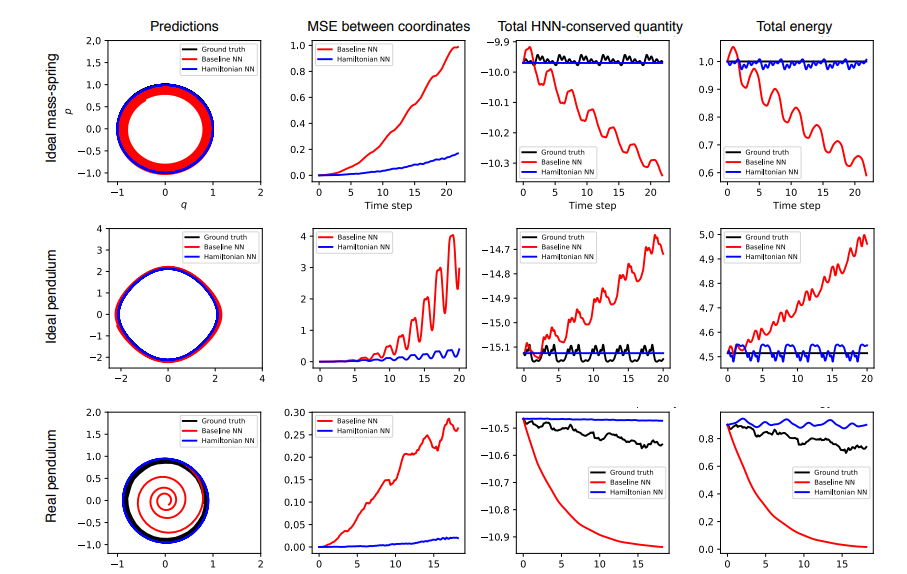
\includegraphics[width=\linewidth]{pendulum.png}
  \centering
\end{figure}

\begin{figure}[H]
  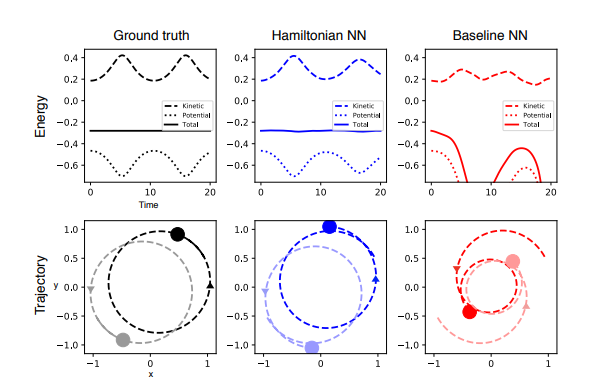
\includegraphics[width=\linewidth]{twobody.png}
  \centering
\end{figure}

Beyond energy conserved system, we could also try to extend to nonconservative system, such as damped SHM (linear perturbation (dissipative system)) or nonlinear pertubation.
We can write damped harmonic oscillator's Hamiltonian can be written as $$
H=\frac{m \dot{x}^{2}+k x^{2}}{2} e^{\alpha t}, 
$$ 
we just have to treat the problem as time dependent add add that as one of our variable and the its dynamics will be unity.
It is not invariant, but we know its change with respect to time.
Or we can write it in a different coordinate $X=x\exp(\alpha t/2), P = p\exp(-\alpha t/2)$, and make it a time independent Hamiltonian.
For nonlinear pertubation, such as $x^3$, the resulting phase portrait still have periodic orbits.
If we have something like Van der Pol oscillator, then we will have limit cycles, the Hamiltonian is not conservered but again we can write it as time independent Hamiltonian.
The energy is conserved over a cycle.
We can also consider duffing oscillator.
In dissipative system, momentum can still be preserved. 
Or for some system, conservation of flow and mass (total derivative is zero).
Actually, we probably doesn't even need to write it as a Hamiltonian since we are not using any property of it.
The two most important ingredients for the procedure to work is invariance (or invariance after time is taken as a variable) as well as periodicty (normal orbit or limit cycle).
Dissipative system has the former but not latter.
Van der pol has later and former in a different form (invariance over a cycle)
Duffing equation also have the latter but not the former (besides special case parameter values). 
Require two time scales for good approximations for weakly nonlinear oscillator.
If period can also be paramertised as a function of energy, we can backpropagate to learn it.
Invariance is important since we are essentially using it to index our trajectories, and because it's invariant, it can be used throughout the process. 
Is it worth to look into topology and manifolds?

I am thinking we can parametise the invariance with neural network or even just a linear operator (since non linear one can be approximate with linear near fixed point), so that we paramertise with the linear coefficients, then we can backpropagate to learn it.  

Can we also use Liouville theorem to encode data uncertainities? invariance in phase space volume.

\section*{Dynamical system textbook finding}
\begin{enumerate}
\item For nonlinear system, we can linearlise the model about the fixed point (essentailly the small energy pertubation approximation), using Taylor expansion and keep the first order term in the Jacobian matrix. $=>$ therefore, if our $\mathbf{f}$ is not linear, we can approximate it with $\nabla \mathbf{f}$ for small pertubation. We can then learn the Jacobian and invert it to get the original $\mathbf{f}$. 

\item The phase space trajectories do not intersect $=>$ probably not very useful.
\item Now I think the invariance should hold throughout the phase space and I have to work out the details of the proof.
\item Can we consider learning the potential instead of the total energy? $=>$ probably not very useful
\item Another property of a conservative system is that typically they have closed trajectories (contours of constant energy). $=>$ so they are always periodic
\item We may perhaps learn the dyanmics from energy surface? $=>$ If we know the energy surface (by learning invariance), we will automatically get the dynamics from the horozontal cut.$=>$ I think this is quite useful, so that we will condition on the energy being constant and then we can get the dynamics automatically.
\item Since the loops are closed, they are usually periodic, besides special points, so my argument of assuming periodcity applies. However, at different trajectory, they may have different period. $=>$ if we know they are on the same energy level, the periodicity should be the same. (Therefore, we should have a periodicity kernel that depends on the energy?) $K = \sigma^2 \exp\left(-\frac{2}{l^2}\sin^2\left(\pi \frac{|x-x'|}{p}\right)\right)$. The energy will control the periodicity p. How to enforce that? We know that if the energy is different, we should have low covariance anyways, if we have same energy, we will have same periodicity. 
\item Can we also consider reversibility as a symmetry? $=>$ don't think it's very helpful but may speed up training by half? or as some sort of constraint?
\item Index invariance $=>$ may be too involved in dyanmical theory to be useful, and mostly likely not. 


\end{enumerate}
\iffalse
\section*{Rough future plans?}
\begin{enumerate}
  \item Assume known invariance, derive dynamics using conditioning
  \item Assume known invariance, derive dynamics using conditioning and the special kernel
  \item Assume unknown invariance, do the above by paramertising invariance and maximise marginal likelihood
  \item If all of the above works, extend to system with nonlinear dynamics (i.e. Van der Pol, Duffing (double well), dissipative )
\end{enumerate}
\fi
\section*{Summary for next meeting}
\begin{enumerate}
  \item We established that the invaraince should hold throughout the phase space
  \item Do we condition on the entire grid points in that case? How does conditioning works?
  \item In higher dimensions, simple conservation of energy can only constrain the dynamics but not determine it uniquely
  \item energy conservation kernel and spatially frequency varying periodicity kernel? energy as index of the trajectory
  \item Low energy pertubation, and linearlising dynamics around fixed point
  \item Hamiltonian NN
  \item time dependent Hamiltonian with time being an extra variable
  \item weakly non linear system and two time scales method
  \item paramertising invariance with NN?
  \item energy surface countours are the same as dynamics
  \item invariance manifolds
  \item 
\end{enumerate}

\end{document}

